\section{Introduction}
Particle Swarm Optimization (PSO)\cite{pso} is a computationally intensive algorithm for
global optimization that quickly becomes intractable for
high-dimensional search spaces and large numbers of particles when run
sequentially. To overcome this limitation, practitioners turn to parallel
implementations, which typically rely on placing locks on the global best
particle (\texttt{gbest}) or through the use of sub-swarm techniques. In this
work we introduce a cache-aware, lock-free parallel PSO algorithm that uses a
shared \texttt{gbest} vector. Our experimental results show over a $6\times$
runtime improvement in some scenarios in addition to demonstrating better
scalability then both the object-oriented and cache-aware implementations.

The primary challenge in parallelizing PSO is handling the update of
\texttt{gbest}. The prevailing approaches are to lock \texttt{gbest} during a
write or to use a sub-swarm based technique. The lock-based approach shows the
worst scalability in the parallel setting due to the high cost of repeatedly
acquiring and releasing the lock, in addition to the challenge of writing
correct, bug-free code involving locks. To get around this issue, researchers began
studying sub-swarm-based approaches. The sub-swarm algorithms still require a
way in which the sub-swarms share information about their sub-swarm best; this
is typically done via a shared resource, which requires locking, or via some
form of message passing.

While sub-swarm techniques alleviate some of the scalability problems of
lock-based approaches, they still suffer from requiring locks in the
shared-resource setting
or increased program complexity in the form of special sub-swarm topologies
and/or communication patterns. The shared-resource approach uses some type of
single \texttt{gbest} that is periodically updated by the sub-swarms, which
requires some form of locking. This locking can be avoided by introducing some
form of message passing, typically with a specialized swarm/sub-swarm topology
introduced to reduce the number of messages being sent (e.g., in the naive
approach where every particle sends a message to every other particle, there are
$O(n^2)$ messages for $n$ particles).

The essence of our algorithm is allowing the system of particles to occasionally
make irrational steps---steps that are in a direction other than that dictated by
standard PSO---with the goal that this relaxed algorithm has a reduced runtime.
This is done by reducing the randomness in the velocity updates and
allowing non-atomic reads of \texttt{gbest}. Using non-atomic reads and writes
is particularlly interesting because it means the system might use values of
\texttt{gbest} that are non-sensical. Although this is troubling from a
correctness standpoint, the performance characteristics are quite impressive.

The contributions of this work are:
\begin{itemize}
\item A lock-free, cache-aware algorithm for parallel PSO
\item Confirmation of previously achieved results by Chang et
  al. \cite{cache-pso}
\item A modified PSO algorithm that reduces stochasticity of velocity updates
  but gains improved runtime performance.  
\end{itemize}

The organization of this paper is as follows. Section \ref{sec:pso} gives a
brief overview of PSO followed by Section \ref{sec:cache}, which describes
cache-aware algorithms and introduces the concept of data-oriented design. In
Section \ref{sec:results} we discuss experimental results. Finally, in Section
\ref{sec:prior} we discuss prior work.


\section{Related Work}\label{sec:prior}
There is a large body of work studying the parallelization of PSO. This work can
be broadly broken up into two categories: OpenMP/MPI based methodoligies and
GPGPU based methodoligies (typically via CUDA). OpenMP is a set of pragmas used
with C/C++ or Fortran that automates much of the multi-threading process. MPI
(Message Passing Interface) is an API for C and Fortran (among others) that
allows communication between independent processes. Within the OpenMP and MPI
context, each process or thread can perform a completely unrelated task to the
other processes or threads without loss in performance. CUDA's computational
model is much more strict; optimal thread efficiency is generally achieved when
all GPU threads are performing the same action. While branching within the
kernel is allowed, if thread branches diverge (i.e., threads take different
branches), performance is dramatically reduced as the GPU is only capable of
performing one branch at a time. The reduced computational flexibility of the
GPU is offset by massive parallelism -- commodity GPUs can have upwards of 4,000
threads on a single card.

Using OpenMP and MPI is the simplest approach to parallelizing PSO. Within the
OpenMP/MPI domain, several architectures emerge: sub-swarm-based, fitness
function-based, and particle-based. While the algorithms themselves vary, these
architectures all share the same core mechanic where MPI handles inter-node
communication of globally shared state and OpenMP handles intra-node parallelism
via threading.

Sub-swarm architectures break the initial set of particles into so-called
``sub-swarms''. Nedjah et al. \cite{comppso} use these sub-swarms to explore
low-dimensional and orthogonal subspaces of the initial search space. However,
the gain from reducing the dimensionality is partially offset by fitness
evaluation, which requires communication across all swarms. Due to the high
communication cost of the fitness function evaluation, this approach does not
scale well to large sytstems. Chang et al. \cite{ppso} note that when a fitness
function can be optimized independently across its dimensions the sub-swarms can
work independently with minimal communication. When this isn't the case, they
propose a semi-synchronized algorithm that updates \texttt{gbest} across all
threads every fixed number of steps. Peng et al. \cite{multicore-pso} also
investigate the sub-swarm approach to
parallelization but explore several different swarm communication topoligies and
use Java threading rather than OpenMP and MPI.

Sub-swarm approaches work well for problems with a relatively inexpensive
fitness function evaluation. However, evaluating the fitness function across all
particles can be computationally expensive; in these cases, performing the
fitness function evaluation in parallel can offer improvement. The parallel
fitness function architecture \cite{pgpso, ppso-fd} uses a coordinator process
to handle the PSO update and sends particle data to worker processes that
evaluate the fitness function for the given particle. These worker processes are
frequently multi-threaded via OpenMp.
This works well for a small number of particles, but communication
overhead will quickly dominate large systems of particles. In the case of large
systems of particles, it may be more efficient to utilize a sub-swarm approach.

Similar to the parallel fitness function evaluation, several works
\cite{cooppso, optionpso} distribute individual particles to worker nodes. Each
worker node is responsible for performing the PSO algorithm on its single
particle and sending particle information to a coordinator node after each
iteration. The coordinator uses the collected information to determine
\texttt{gbest} and broadcasts it to the system. While this broadcast can be done
efficiently in $O(\lg n)$ time depending on the system network, overall this
approach suffers from poor scalability due to the high communication overhead
and blocking nature of the algorithm. In this case, the system is only as fast
as its slowest node (a common problem with MapReduce algorithms as well).

The most unique approach to parallelizing PSO via OpenMP and MPI is by Koh et
al. \cite{papso} which proposes an asynchronous, distributed PSO implementation
based on a shared queue of particles. 

Another common approach to parallelizing PSO is via GPGPU programming
\cite{gpu-ppso, gpu-pso, biopsogpu}. GPU-based
algorithms primarily use the GPU for fitness function evaluation, although
some are able to perform the entirety of the PSO aglorithm on the GPU
\cite{swarmgrid, multiswarmpso-gpu}.
% The
% challenge with GPGPU programming is two-fold: minimizing communication between
% the GPU and CPU, which is costly, and avoiding branching within the GPU
% kernel\footnote{a kernel in GPGPU programming is the name of the procedure being
%   run on  the GPU}. When grouped threads (referred to as a warp) within a GPU
% start to diverge due to branching, the
% GPU executes one branch at a time.
% This can be difficult to avoid in the PSO algorithm where a core part
% of the aglorithm is finding the globally optimal particle (i.e., \texttt{gbest}).
% To get around this,
% some work \cite{gpu-ppso, gpu-pso, biopsogpu} uses the GPU primarily for evaluating the
% fitness function across all particles simultaneously.
% Others \cite{swarmgrid, multiswarmpso-gpu}, perform the entirety of
% the PSO algorithm on the GPU, transferring data from the CPU to the GPU at the
% beginning of the algorithm and then transferring the data back to the CPU from
% the GPU at the end of the algorithm. Updates to \texttt{gbest} are performed at
% a set interval.

Other recent work \cite{mrcpso, mprso, coop-pso, intrusion-pso} has
studied the use of the MapReduce framework \cite{mapreduce} in parallelizing PSO
for various applications.
% In most experiments, these works see near linear
% scaling with number of nodes added in the MapReduce cluster.
% The MapReduce implementations serve as a complementary
% approach to the CPU and GPU-based work. For example, each node in the MapReduce
% cluster can run an OpenMP and/or
% GPGPU-based algorithm. Improvements to the CPU and GPU PSO algorithms directly
% flow into the work of the MapReduce-based algorithms.
A similar approach of using
MapReduce for coarse-grain parallelism and resiliency while allowing
models to manage the fine-grained
parallelism is also being investigated by the deep learning community \cite{mrpnn,
  heterospark, dlspark}. 


\section{Particle Swarm Optimization}\label{sec:pso}
Particle Swarm Optimization (PSO) \cite{pso} is a global optimization technique
inspired by swarm behavior found in nature (e.g., a flock of birds).
Each particle in the swarm moves in a stochastically weighted
combination of two vectors: one in the direction of the best location the
particle has seen locally and one in the direction of the best location seen by
the swarm globally. Here the term ``best'' is with respect to a predefined and
problem specific fitness function.
The swarm maintains a global best position (the position
with the optimal fitness value) and the goal is for this global best position to
converge to the global minimum (maximum).
One of the characteristics of PSO is that it searches globally for the optimum,
although it does not have a guarantee of convergence.
In particular, if the particles are initialized in a subspace far from the
global optimum, the change of convergence is greatly reduced.

Particle Swarm Optimization can be simplified into the update of two formulas:
one for a particle's velocity and the other for the particle's position. Define
$\textbf{pbest}$ as the position corresponding to the best seen fitness value
for a given particle (i.e., the local best), $\textbf{gbest}$ as the position
corresponding to the the best seen fitness value globally, and $\textbf{p}$ as
the current position of the given particle. The update formula for velocity is
given by equation (\ref{eq:velocity} and Table \ref{tab:constants} describes
the interpretation of the constants.

\begin{align}
  \textbf{v}_i(t+1) = \omega \textbf{v}_i (t) & +
                                                c_1 \textbf{r}_1\odot (\textbf{pbest}_i(t) -
                                                \textbf{p}_i(t))
  \\\label{eq:velocity}
  &+ c_2 \textbf{r}_2 \odot(\textbf{gbest}_i(t) - \textbf{p}_i(t))\nonumber
\end{align}

Where $\odot$ is the Haddamard product.
Once the velocity is computed, the position update is given by equation
(\ref{eq:position}).

\begin{equation}\label{eq:position}
  \textbf{p}_i(t+1) = \textbf{p}_i(t) + \textbf{v}_i(t)
\end{equation}

\begin{table}
  \caption{Description of the velocity update constants.}\label{tab:constants}
  \begin{tabular}{ll}\toprule
  \textbf{Constant} & \textbf{Description}\\\midrule
  $\omega$ & Momentum\\
  $c_1$ & Explore towards local best\\
  $c_2$ & Exploration towards global best\\
  $r_1$ and $r_2$ & sampled from $U(0,1)$\\\bottomrule
  \end{tabular}
\end{table}

Algorithm \ref{alg:pso} describes the basic PSO algorithm.

\begin{algorithm}
  \caption{Basic PSO algorithm.}\label{alg:pso}
  \begin{algorithmic}[1]
    \Procedure{PSO}{N}
    \State $\texttt{particles} \gets \texttt{initialize}(N)$
    \Repeat
    \For{$\textbf{p} \in \texttt{particles}$}
    \State $\textbf{gbest} \gets \arg\min_{p\in\texttt{particles}}f(p)$
    \State \texttt{p.UpdateVelocity(\textbf{gbest})}
    \State \texttt{p.UpdatePosition()}
    \EndFor
    \Until Convergence
    \EndProcedure
  \end{algorithmic}
\end{algorithm}

Particles are initialized randomly within the bounds of the search space
$[\texttt{x\_min}, \texttt{x\_max}]$. Particle intialization is an important
step -- if the global optimum is far outside the initialization domain, the
algorithm may not converge to the global optimum.
Some implementations also set a random
intiail velocity for each particle; however, we found it simpler and equally
effective to initialize all particles with zero velocity. In our initial
experiements, we found improved convergence by reflecting particles off the
boundary of a predefined search space using $[x_{\min}, x_{\max}]$. The
reflection was performed by negating the velocity component and offsetting the
particle from the boundary by the amount it would have exceeded the boundary for
the respective position component.
However, we decided to use an open search space with no boundary to give a more
pessimistic view of our algorithm.

Our implementation allows for a predefined minimum and maximum value for
components of the velocity vector -- in practice these should be no greater than
the diameter of the search space.


\section{Cache-aware Algorithms}\label{sec:cache}
Modern x86\_64 CPUs typically have three tiers of cache: L1, L2, and
L3. L1 cache is the fastest but has the smallest amount of storage and L3 is the
slowest but has the largest amount of storage.
When data is to be loaded into a register, the CPU first checks the
cache, then RAM, and lastly disk. Rather than load a single piece of data from
RAM (or disk) into cache, the CPU loads a cache line, which is typically
64B. For 32-bit numbers, this cache line corresponds to 16 values and eight
values for 64 bit number.
A cache-aware
algorithm utilizes this information by grouping data such that data utilized by
the algorithm in temporal proximity is stored physically close together
\cite{scientific-software}. This
is referred to as data locality. In other words, we want to keep data that is
accessed at around the same time as close together as possible. Doing so reduces
access to RAM and disk, both of which are substantially more
costly than accessing cache.

\subsection{Data-Oriented Design}
We can use the idea of data locality to
influence the design of our programs. This is one aspect of what is known as
data-oriented design\cite{dod} and
is a very common technique in the video game industry, which is known for
writing performant code.
Data-oriented design
differs from object-oriented design in that data is grouped based on access
paterns rather than logical patterns.

\begin{figure}
  \lstinputlisting{../code/particle.cpp}
  \caption{Example of a Particle class using object-oriented
    design.}\label{fig:particle}
\end{figure}

Figure \ref{fig:particle} shows a typical object-oriented implementation of PSO.
The information specific to a particle is logically grouped together. From a
design point of view, this is a sensible approach. However, as we will
demonstrate in the experiments section, this design choice reduces performance
for highly sequential access patterns (such as PSO).
When a particle gets loaded into cache, the
cache line will contain three pointers to \texttt{T}, which is either a
32-bit or 64-bit floating point number, the three constant values
$c_1$, $c_2$, and $\omega$, and three function pointers to the fitness,
position, and velocity update functions.

Figure \ref{fig:particles} shows one possible data-oriented design
approach. Notice that the particle attributes--position, velocity, particle
best--are split across three separate vectors. CPU
assumes (hopes) a load from one address will be followed by loads from nearby
addresses and, in the case of 64-bit floats, will pull the next seven values in
memory into cache. Because we structured our data to use these values next, the
CPU saves as many as seven memory accesses.

Both the object-oriented and data-oriented designs store velocity and position
data as vectors. Since both design approaches share this aspect, we may be left
wondering why the data-oriented design is more efficient. First, in the
data-oriented design, the first load is the vector pointer, which is then
followed by successive loads corresponding to element access. However, that
initial load pulled in the vector pointer for the current vector as well as the
vector pointers for the next seven pointers (assuming a 64-bit system). This is
not the case in the object-oriented design because the object contains pointers
to velocity, position, best position, constant values, and function
pointers. Thus it is unlikely a load of one vector pointer will contain the
pointers of successive vectors.

Another aspect that hurts the object-oriented performance is the cache eviction
caused by the extra data contained in the cache line. Some of this data is not
used during particle updates and takes up valuable cache space. In some cases,
this data may even evict data from the cache that will be needed in the near
future. Using the design illustrated in Figure \ref{fig:particle}, each cache
line resulting from a particle load will have over 11\% wasted space due to the
fitness function pointer alone (of the nine values loaded, the fitness function is
not used and thus is wasted space). Also note that the call to
\texttt{UpdateVelocity} will iterate over the velocity vector, bringing in
elements of the velocity vector into cache and possibly evicting the function
pointer for the \texttt{UpdatePosition} method. This eviction will cause another
expensive access to main memory. Avoiding this waste is what makes the
data-oriented approach so efficient.


\subsection{Terminology}
The object-oriented design is sometimes referred to as \emph{array of structs} (AoS) while
the data-oriented design is referred to as \emph{struct of arrays} (SoA). This
terminology is intuitive; an array of structs is a more generic term for a
vector of objects, while a struct of arrays is a generic term for an object
containing vectors.
We use this terminology and add a third: SoA-fast, which
represents the efficient, data-oriented design. These names are summarized in
Table \ref{tab:names}

\begin{table}
  \centering
  \caption{Description of algorithm names.}
  \label{tab:names}
  \begin{tabular}{ll}\toprule
    \textbf{Name} & \textbf{Description}\\\midrule
    AoS & Array of Structs - Object Oriented\\
    SoA & Struct of Arrays - Data Oriented\\
    SoA-fast & Efficient Struct of Arrays\\\bottomrule
  \end{tabular}
\end{table}

          

\begin{figure}
  \lstinputlisting{../code/particles.cpp}
  \caption{Example of a data-oriented design modeling all particles in a PSO
    simulation.}\label{fig:particles}
\end{figure}

\begin{algorithm}
  \caption{Cache-aware algorithm for PSO.}\label{alg:pso-cache}
  \begin{algorithmic}[1]
    \Procedure{PSO-DO}{N}
    \State $\texttt{vel} \gets \texttt{initialize}(N)$ \Comment{velocity vectors}
    \State $\texttt{pos} \gets \texttt{initialize}(N)$ \Comment{position vectors}
    \State $\texttt{bpos} \gets \texttt{pos}$ \Comment{best position vectors}

    \Repeat
    \State $\texttt{gbest} = \text{argmin}_{\texttt{pos}}\texttt{fitness}(p)$
    \For{$i = 0 \to \texttt{n\_particles}$}
    \State $p \gets \texttt{pos}[i]$
    \State $v \gets \texttt{vel}[i]$
    \State $\texttt{local} \gets (\texttt{pos}[i] -
    \texttt{bpos}[i])$
    \State $\texttt{global} \gets  (\texttt{pos}[i]
    - \texttt{gbest})$
    \State $v \gets \omega v + c_1 r_1 \texttt{local}  + c_2 r_2 \texttt{global}$
    \State $p += v$
    \If{$\texttt{fitness}(p) < \texttt{bpos}[i]$}
      \State $\texttt{bpos}[i] \gets p$
      \If{$\texttt{fitness}(p) < \texttt{fitness}(\texttt{gbest}$}
      \State $\texttt{gbest} \gets p$
      \EndIf
    \EndIf
    \EndFor
    \Until convergence
    \EndProcedure
  \end{algorithmic}
\end{algorithm}

\section{Cache-aware Parallel PSO}\label{sec:algo}
We make several improvements to the framework for cache-efficient PSO proposed
in \cite{cache-pso}. While none of these improvements is a major structural
change to the algorithm of PSO or the data-oriented design, we found that the
net effect was a dramatic improvement in performance.

\begin{figure}
  \lstinputlisting{../code/naive_par.cpp}
  \caption{Naive random weight generation.}\label{fig:naive-par}
\end{figure}

\begin{figure}
  \lstinputlisting{../code/efficient_par.cpp}
  \caption{Efficient random weight generation.}\label{fig:efficient-par}
\end{figure}

\subsection{Random Weights}
One of the major speed-ups we achieved was through
the generation of the random weights $r_1$ and $r_2$. The original description of
PSO \cite{pso} has two calls to \texttt{rand()} during the velocity update for each
component of the velocity vector. We surveyed a number of highly cited works in
PSO literature \cite{pso-development, pso-overview, pso-tutorial} and found in
all descriptions of the algorithm the random values $r_1$ and $r_2$ are sampled
for each element of $\textbf{v}$ (i.e., for $\textbf{v}\in\mathbf{R}^n$ there
are $n$ unique values of $r_1$ and $n$ unique values for $r_2$). We modify this
approach to use a single value $r_1$ and a single value for $r_2$ for all
components of \textbf{v}. Additionally, in the effecient implementation, we batch
the generation of these values once per system update, rather than generating
them for each vector.
There are two advantages to this approach: we can keep
these random values in cache and we avoid expensive calls to random number
generation routines. This can be seen in Figures \ref{fig:naive-par} and
\ref{fig:efficient-par}. The naive approach, shown in Figure \ref{fig:naive-par}
makes two calls to
\texttt{random\_uniform} for each particle. The efficient approach, shown in Figure
\ref{fig:efficient-par},
indexes the $r$-value vectors \texttt{r1s} and \texttt{r2s}, which are
created at the start of each call to \texttt{UpdateVelocity}. This is a rather
obvious optimization; however, in
practice it seems it is an optimization that is frequently overlooked.
Another potential criticism of this approach is that it reduces variation in the
updated velocity, which could potentially slow convergence. In our experience,
the speed-up gained by using a single $r_1$ and $r_2$ outweighs any slowed
convergence resulting from reduced diversity.\par
We could further improve performance be passing in a pre-allocated vector to the
random number generating routine. However, this makes the code a little more
opaque since it is not always clear a return parameter is returning a
value. Additionally, it is possible that in some cases the compiler is eliding
this allocation on its own.

\subsection{Reducing Critical Section Contention}
Updating \texttt{gbest}
requires checking all particles against the current \texttt{gbest} and updating
when a position with a better fitness value is found. This is a classic
reduction scenario, which can be done in $O(\lg n)$ time. OpenMP provides the
facilities to handle this efficiently, but only for a few simple types and
operations. Unfortunately, these do not include \texttt{std::vector<T>}. Similar to
prior works, we do a linear scan of all particles in parallel. This presents its
own challenge due to the data race that occurs when multiple threads attempt to
read or write \texttt{gbest}. Figure \ref{fig:naive-update} shows an example of a
standard use of OpenMP's \texttt{critical} section to avoid the data race.
Performance is reduced due to hitting the critical section for every particle on
every update. We use two nested if-statements
with the critical section on the inner statement, as shown in Figure
\ref{fig:efficient-update}. The intuition behind this is quite simple -- rather
than take a hit on the critical section for every single particle, we
have all particles first check if they could possibly be the best global
partical by checking against the current \texttt{gbest}. If this fails, they
miss the critical section and move on. In the even the first check passes, the
particle then hits the critical section. As demonstrated in our
experiements, this produced a substantial speed-up.

Although we are able to avoid ctirical section contention for a number of the
particles, the careful reader will note we have not protected against reads
during a write to \texttt{gbest} (i.e., the writes are not atomic).
This has two primary
consequences. First, some particles may use an incorrect \texttt{gbest} when
computing the velocity update -- this can occur if they read \texttt{gbest}
while another thread is updating \texttt{gbest}. Second, some particles that are
currently the true \texttt{gbest} may skip the critical section if they read an
incorrect value of \texttt{gbest} that results in a lower fitness value. Both of
these issues result in a slower rate of convergence. Despite the slower rate of convergence,
the actual wall-clock time is substantially faster. Similar to the asynchronous,
distributed deep learning algorithms \cite{adam, downpour}, we trade reduced convergence for
faster runtime.


\begin{figure}
  \lstinputlisting{../code/naive_update.cpp}
  \caption{Naive update in a critical section for the naive parallel PSO
    algorithm.}
  \label{fig:naive-update}
\end{figure}

\begin{figure}
  \lstinputlisting{../code/efficient_update.cpp}
  \caption{Efficient update in a critical section for the efficient parallel PSO
    algorithm.}
  \label{fig:efficient-update}
\end{figure}


\begin{algorithm}
  \caption{Cache-aware parallel PSO}\label{alg:par-pso}
  \begin{algorithmic}[1]
    \Procedure{Parallel-PSO}{N}
    \State $\texttt{n\_threads} \gets \texttt{getn\_hardware\_threads}()$
    \State $\texttt{tp} \gets \texttt{ThreadPool}()$
    \State $\texttt{vel} \gets \texttt{initialize}(N)$
    \State $\texttt{pos} \gets \texttt{initialize}(N)$
    \State $\texttt{bpos} \gets \texttt{pos}$

    \State $n = N/\texttt{n\_threads}$ \Comment{Assume $N \mod
      \texttt{n\_threads} = 0$}
    \For{$(i, t) \in \texttt{enumerate}(\texttt{tp})$}
    \State $vs \gets \texttt{vel}[ni:n(i+1)]$
    \State $ps \gets \texttt{pos}[ni:n(i+1)]$
    \State $bps \gets \texttt{bpos}[ni:n(i+1)]$
    \State $t \gets \texttt{Thread}(\texttt{Run},vs, ps, bps)$
    \EndFor
    \Comment{Wait for threads to finish}
    \For{$t \in \texttt{tp}$}
    \State \texttt{t.join()}
    \EndFor
    \EndProcedure
  \end{algorithmic}
  \begin{algorithmic}[1]
    \Procedure{Run}{\texttt{vs}, \texttt{ps}, \texttt{bps}}
    \State \Comment{\texttt{gbest} is shared between the threads}
    \State $n \gets \texttt{ps.size()}$
    \Repeat
    \For{$i = 1 \to n$}
    \State $v \gets \texttt{vs}[i]$
    \State $p \gets \texttt{ps}[i]$
    \State $bp \gets \texttt{bps}[i]$
    \State $\texttt{UpdateVelocity}(v, \texttt{gbest})$
    \State $\texttt{UpdatePosition}(p, v, bp, \texttt{gbest})$
    \EndFor
    \Until convergence
    \EndProcedure
  \end{algorithmic}
\end{algorithm}


\section{Results}\label{sec:results}
\begin{table}
  \centering
  \caption{Test functions used in experiments.}\label{tab:functions}
  \begin{tabular}{ll}\toprule
    \textbf{Name} & \textbf{Function}\\\midrule
    Ackley & $-20\exp\Big(-0.2\sqrt{\frac{1}{n}\sum_ix_i^2}\Big)$ -\\
    & \hspace{5mm} $\exp\Big(\frac{1}{n}\sum_i\cos(2\pi x_i)\Big) + e + 20$\\
    Quadratric & $\sum_i x_i^2$\\
    Rastrigin & $10n + \sum_{i=1}^n(x_i^2 - 10\cos(2\pi x - i))$\\\bottomrule
  \end{tabular}
\end{table}
We test our algorithm on several popular test functions in optimization
\cite{testprobs} the the quadratic, Rastrigin
\cite{rastrigin}, and Ackley \cite{ackley} functions, shown in Table
\ref{tab:functions} generalized to $\mathbb{R}^n$. All of these functions have
the property that their minimum is attained at the origin with a value of
$0$, which makes assessing the models easy. Three-dimensional plots of the
Rastrigin and Ackley functions are shown in Figures \ref{fig:rastrigin} and
\ref{fig:ackley}, respectively.
All experiments were run on a single
workstation with a 6-core, 3.6 GHz Intel i7-6800K processor and 64GB of RAM. We
used six threads in OpenMP, rather than 12 hyperthreads, to reduce context switching.
Table \ref{tab:param}
gives the hyperparameters used in the experiements, which were chosen based on
the recommended values from \cite{pso-convergence, spso} -- the advantage of
using these parameters is that they do not need tuning. It is
worth noting that in our experience these parameters work well but performance
can frequently be improved via tuning.

\begin{table}
  \centering
  \caption{Hyperparamters used in the experiements.}\label{tab:param}
  \begin{tabular}{lc}\toprule
    \textbf{Parameter} & \textbf{Value}\\\midrule
    $c_1$ & $2.05 \chi$\\
    $c_2$ & $2.05 \chi$\\
    $\omega$ & $\chi$\\
    $\chi$ & $\frac{2}{2.1 + \sqrt{.41}}$\\\bottomrule
    \end{tabular}
\end{table}

Bratton et al. \cite{spso} mention that particles should be initialized away
from the target global optimum to prevent unintentional bias as a result of
particles being initialized close to the optimum. However, since our
distributions have their optimums at the origin, moving to a higher dimensional
space means that particles randomly intialized from a uniform distribution will
cluster towards the outer edges of the search space (see, for example, ``curse
of dimensionality'' \cite{hastie}). Empirically, in $\mathbb{R}^{10}$, the
probability a point being randomly initialized within $\text{diam}/2$ of the origin is 0.1 \%.
We verified this experimentally and found no
impact to runtime when sampling initial positions from $U(x_{\min}, x_{\max})$
and from $U((x_{\min},\lambda x_{\min})\cup(\lambda x_{\max}, x_{\max}))$.


\begin{figure}
  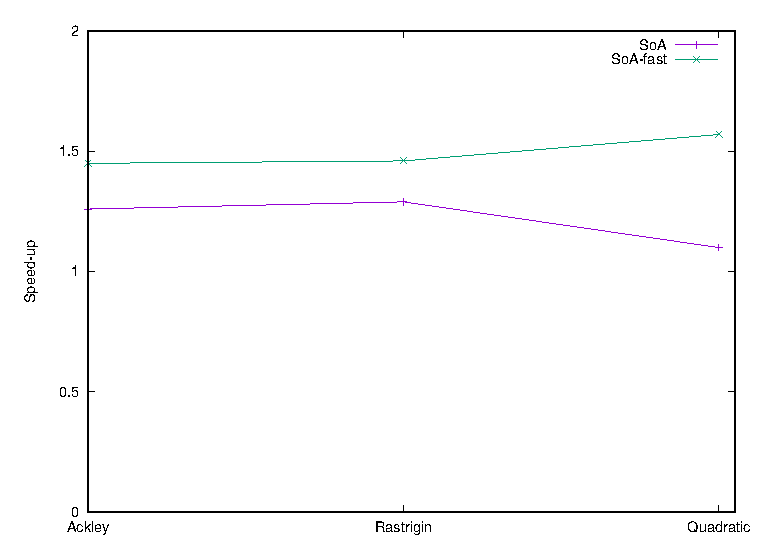
\includegraphics[width=\columnwidth]{../img/output/speedup_seq}
  \caption{Speed-up over AoS in the sequential setting.}\label{fig:seq-baseline}
\end{figure}

% \begin{table}
%   \centering
%   \caption{Sequential speed-up with respect to Array of Structs design (dimension
%     75 with 500 particles.)}
%   \label{tab:seq-baseline}
% \begin{tabular}{llll}\toprule
% Structure       & Ackley & Rastrigin & Quadratic \\\midrule
% SoA             & 25.5\%  & 29.2\%     & 10.4\%     \\
% SoA-fast & 44.7\%  & 46.2\%     & 57.0\%     \\\bottomrule
% \end{tabular}
% \end{table}
% 
% Table \ref{tab:seq-baseline} shows the sequential speed-up with respect to the
% AoS design for 500 particles in $\mathbb{R}^{75}$. The SoA architecture as
% proposed in \cite{cache-pso} results in strong improvements over the AoS
% architecture. More interesting is the improvement of the SoA-fast
% architecture. Because these results are for sequential algorithms, the speed-up
% of the SoA-fast algorithm is primarily due to batching the random number
% generation.
% 

Figure \ref{fig:seq-baseline} shows the sequential speed-up ith respect to the
AoS design for 500 particles of dimension 75. The SoA architecture as proposed
in \cite{cache-pso} performs well and shows improved runtimes for all three test
functions. SoA-fast's improvement over SoA is strictly due to the
batching of the random weight generation. Of the three test functions, the
quadratic has the fewest instructions, which means it has the fastest evaluation
time. A side-effect of this is that the SoA-fast architecture sees an
increased speed-up because the PSO algorithm spends a greater porition of its
time in the particle iteration and random number generation parts of the
algorithm and less time evaluating the fitness function.



\begin{figure}
  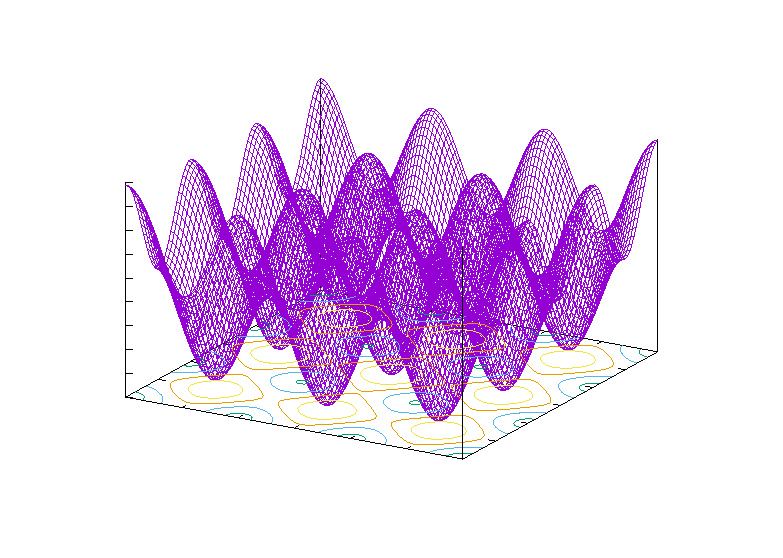
\includegraphics[width=\columnwidth]{../img/output/rastrigin}
  \caption{The Rastrigin function in three dimensions.}\label{fig:rastrigin}
\end{figure}

\begin{figure}
  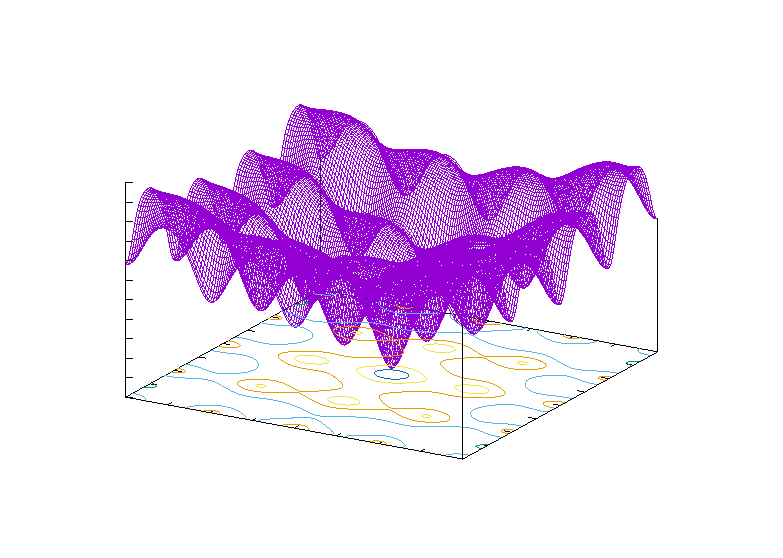
\includegraphics[width=\columnwidth]{../img/output/ackley}
  \caption{The Ackley function in three dimensions.}\label{fig:ackley}
\end{figure}

The batched random weight generations results, while confirmatory, are rather
unsurprising. The more interesting investigation here is how the lack of
consistency guarantees impacts convergence of the SoA-fast algorithm. We
expected the SoA-fast algorithm to require more iterations to converge
but were surprised at how many more iterations were needed in some
scenarios. Table \ref{tab:threshold} summarizes the results of experiments
comparing runtime and steps taken to achieve a desired distance from the
solution. Because we know the solution ahead of time, we are able to measure
both the time and number of steps it
takes for \texttt{gbest} to get within the predefined threshold using the
Euclidean distance metric. For these experiments we use 1,000 particles and
consider the thresholds of 1e-5 and 1e-6; these were chosen because they
gave interesting and reasonable runtimes. We initially experimented with a
runtime of 1e-8 and found that SoA-fast typically failed to converge.

The results in Table \ref{tab:threshold} confirm our hypothesis that the
reducing critical section contention by relaxing consistency
guarantees comes at the cost of reduced convergence efficiency. SoA-fast is
substantially faster than SoA at getting an approximate solution, but for highly
accurate solutions (i.e., low thresholds) the relaxed consistency guarantees
start to dominate the search. For the 1e-6 threshold, SoA-fast is almost
uniformly slower for precisely this reason.

The performance characteristics of SoA and SoA-fast are complementary --
SoA-fast is able to quickly find an approximate solution while SoA is able to
find an accurate solution. These characteristics make for an interesting future
direction of a hybrid approach: a cache-aware algorithm that has relaxed
consistency guarantees initially but switches to a strict consistency regime as
it senses slowed progress.




\begin{table*}[]
  \caption{Comparison of algorithms as a function of solution threshold and
    dimension.}
  \label{tab:threshold}
\begin{tabular}{ccc|cc}\toprule
                                  & \multicolumn{2}{c|}{\textbf{Threshold} $\mathbf{ =
                                    1e-5}$}                         &
                                                                      \multicolumn{2}{|c}{
                                                                     \textbf{Threshold}
                                                                      $\mathbf{ = 1e-6}$}                                          \\\midrule
                   & \multicolumn{2}{c|}{Runtime (s)} &
                                                       \multicolumn{2}{c}{Runtime (s)}\\\midrule
  \textbf{Dimension} & \textbf{SoA} & \textbf{SoA - fast} & \textbf{SoA} & \textbf{SoA - fast}\\
             25              & $0.048 \pm 0.006$   & $0.028 \pm 0.002$  & $0.051 \pm 0.009$    & $0.034 \pm 0.002$   \\
             50             & $0.24 \pm 0.06$     & $0.29 \pm 0.20$    & $1.5 \pm 0.8$        & $2.9 \pm 2.8$       \\
             100         & $15.1 \pm 6.1$      & $13.2 \pm 1.2$     & $55.2 \pm 9.4$       & $82.7 \pm 20.7$    \\\midrule
              & \multicolumn{2}{c|}{Number of Steps} & \multicolumn{2}{c}{Number
                                                      of Steps}\\\midrule
  \textbf{Dimension} & \textbf{SoA} & \textbf{SoA - fast} & \textbf{SoA} & \textbf{SoA - fast}\\
              25        & $229 \pm 15$        & $223 \pm 16$       & $266 \pm 20$         & $271 \pm 18$        \\
             50        & $1,214 \pm 304$     & $2,283 \pm 1,573$   & $7,358 \pm 3,185$    & $22,644 \pm 22,229$ \\
             100       & $52,711 \pm 21,164$ & $96,787 \pm 9,017$ & $193,716 \pm
                                                                    13,855$ &
                                                                              $600,600
                                                                              \pm
  151,416$ \\\bottomrule
\end{tabular}
\end{table*}

% \begin{figure}
%   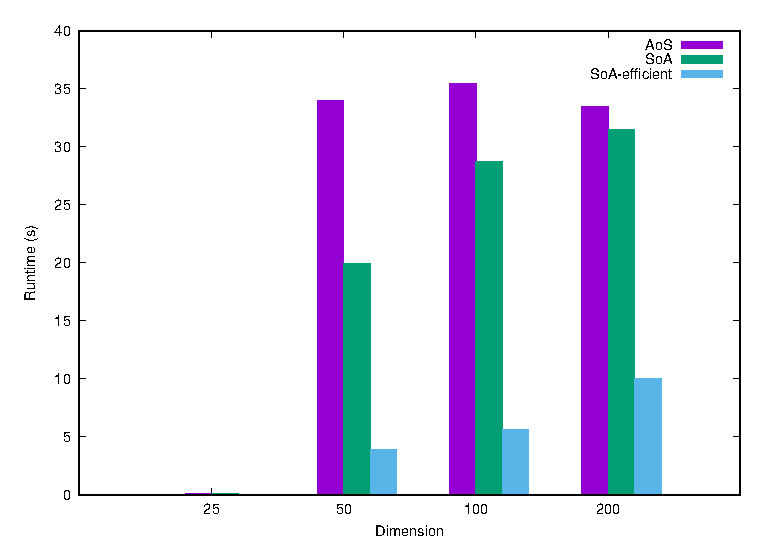
\includegraphics[width=\columnwidth]{../img/output/dim}
%   \caption{Results of the increasing dimension experiments with 1,000
%     particles.}
%   \label{fig:exp-dim}
% \end{figure}
% 
% \begin{figure}
%   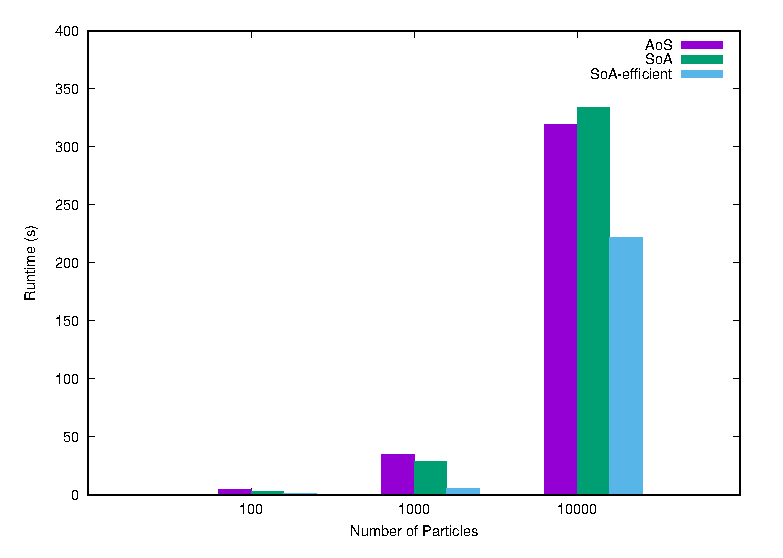
\includegraphics[width=\columnwidth]{../img/output/N}
%   \caption{Results of increasing the number of particles for a fixed dimension
%     size of 100.}
%   \label{fig:exp-N}
% \end{figure}

\begin{figure}
  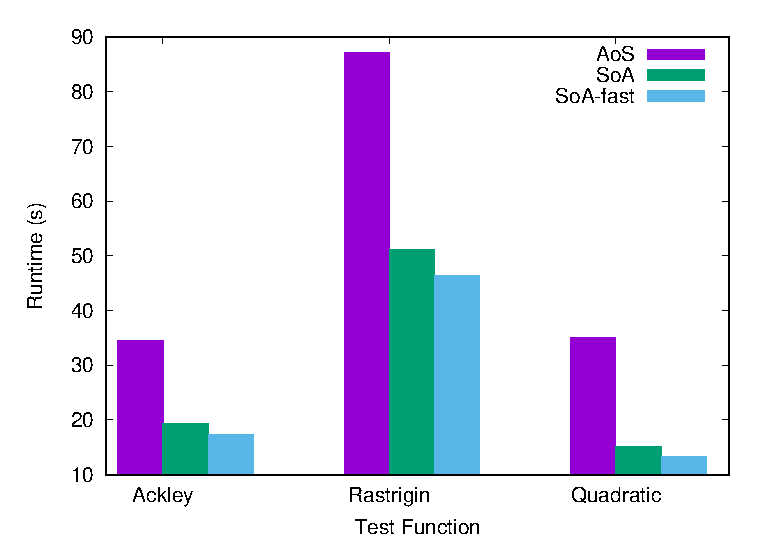
\includegraphics[width=\columnwidth]{../img/output/all3time}
  \caption{Runtime on the three test functions.}
  \label{fig:all3time}
\end{figure}

\begin{figure}
  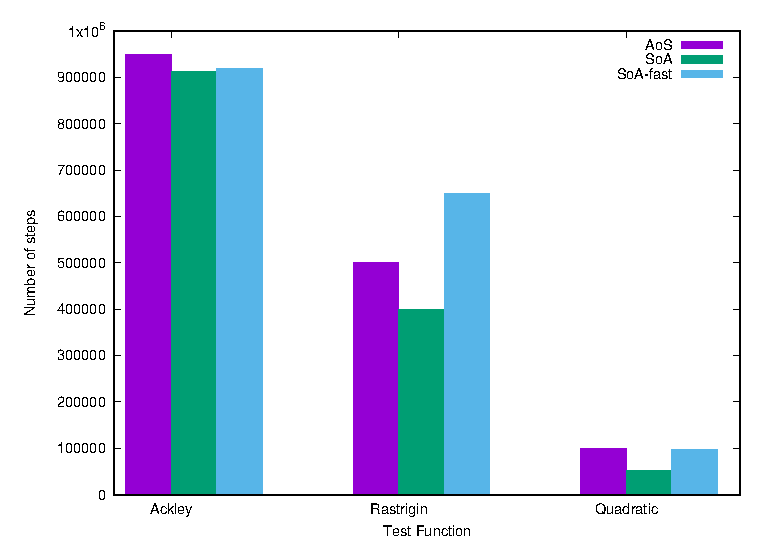
\includegraphics[width=\columnwidth]{../img/output/all3steps}
  \caption{Number of steps to convergence on all three test functions.}
  \label{fig:all3steps}
\end{figure}

\begin{table}
  \centering
  \caption{Summary of test results.}
  \label{tab:results}
  \begin{tabular}{lccc}\toprule
    & \textbf{Ackley} & \textbf{Rastrigin} & \textbf{Quadratic}\\\midrule
    Dimension & 20 & 10 & 100\\
    \# particles & 100 & 500 & 1,000\\
    SoA-fast vs AoS & $2.0\times$ & $1.9\times$ & $2.6\times$\\
    SoA-fast vs SoA & $1.1\times$ & $1.1\times$ & $1.1\times$\\\bottomrule
  \end{tabular}
\end{table}

Figures \ref{fig:all3time} and \ref{fig:all3steps} show the runtime and number
of steps taken for convergence on the three test functions, summarized in Table
\ref{tab:results}.
SoA-fast is about twice as fast as the AoS architecture and
about 10\% faster than the SoA architecture. Similar to the results in Table
\ref{tab:threshold}, SoA-fast consistently requires more steps to converge but
is able to perform those steps faster than SoA and AoS. We want to point out
that these last set of experiments were chosen to showcase SoA-fast's performance.
However, it is important to restate the discussion about Table \ref{tab:threshold}
with respect to the trade-off that makes SoA-fast so performant: the reduced
consistency guarantees of SoA-fast mean it will very quickly (with respect to
wall clock time) converge to an approximate solution, but at a small enough
resolution will fall behind standard SoA.

\section{Conclusion}
In this work we present two optimizations for the performance of both the
standard and parallel version of the PSO algorithm. We introduce
specific guidance on how and where to generate the random weights in
PSO, which, as we demonstrated, results in substantial performance gains. 
The reduced consistency guarnatee of SoA-fast results in around a 10\% performance
gain over the standard SoA architecture. This gain comes at a cost -- SoA-fast
requires more steps (despite a short wall clock time) to achieve a suitable
convergence threshold when compared to SoA. For a small enough convergence
criterion, SoA-fast will struggle to converge. However, for many applications,
SoA-fast converges to a suitable solution in a shorter amount of time. Perhaps
SoA-fast's greatest contribution is that these techniques are easily transferable
to other PSO algorithms, giving PSO implementors two more tricks to add to their
toolbox.


